\chapter{Libro de vida}
\label{cap:librodevida}

El arduo trabajo llevado a cabo en los capítulos anteriores nos ha servido para saber los recursos con los que contamos, pero también con sus limitaciones. Con la experiencia en el entrenamiento de imágenes, decidimos realizar un entrenamiento intensivo sobre una persona para memorar su paso de los años, y de esta manera poder construir el libro de vida personalizado y compuesto exclusivamente con sus recuerdos. Para ello, tomamos como referencia a una persona que tuviera una amplitud de fotografías desde una edad temprana hasta una más avanzada. La persona en cuestión es el actor Alfredo James Pacino, un actor estadounidense de 84 años.


En este punto, vamos a realizar una comprobación de cómo funciona el modelo entrenado de Stable Diffusion con personas en distintas fases de su vida. Lo que queremos testar es que responda bien en todas y cada una de las circunstancias, debido a que para la creación de historias de vida, necesitamos que la persona pueda incorporar imágenes de hechos significativos, que puedan evocar momentos especiales. Para eso se requiere que el modelo funcione bien en todas las etapas, para que la experiencia del usuario pueda ser lo más completa posible.

Vamos a crear 3 entrenamientos diferentes: uno de la persona en su juventud, otro de la persona en la edad adulta y otro de la persona en su edad anciana. Resaltamos que el hecho de que la persona esté incorporada en Stable Diffusion es indiferente, porque para realizar la prueba se va a nombrar de una manera distinta. Es un nombre que asignaremos que será único, con el fin de que el modelo identifique al elemento entrenado y pueda generar las imágenes personalizadas deseadas. Claro está que en las tres fases se han otorgado diferentes identificadores para que el modelo sepa a cuál de ellas nos estamos refiriendo. Una vez tenemos las 3 capas del modelo entrenadas, decidimos generar 3 imágenes bajo el mismo prompt y parámetros para comprobar la exactitud del modelo. En la figura \ref{fig:3fasesvidaalp} podemos apreciar que los resultados son precisos y con una calidad excepcional.\\
 
El prompt es cuestión fue "Close up studio photo of jovenalp/adultalp/80alp, detail, studio lighting."

\begin{figure}[!htb]
	\centering
	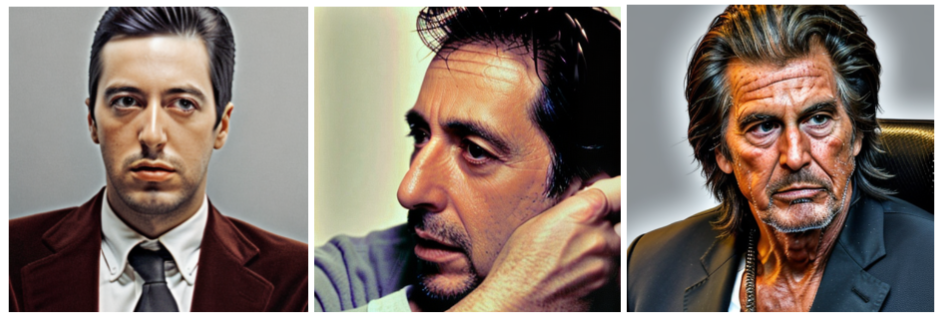
\includegraphics[width = 1
	\textwidth]{Imagenes/Vectorial/3fasesvidaalp.png}
	\caption{Resultados obtenidos bajo un mismo prompt en las 3 fases}
	\label{fig:3fasesvidaalp}
\end{figure}


El objetivo principal de esta tarea es simular una generación de imágenes para un libro de vida de un paciente. Por lo tanto, no solo necesitamos generar fotografías de la propia persona, si no con diversos elementos para cada etapa, para comprobar cómo puede funcionar en la terapia de reminiscencia, cuando se incluyan imágenes personales del paciente, de lugares, personas y otros elementos importantes de su vida.

Para la elaboración del libro de vida se necesita una cantidad considerable de recuerdos y momentos entrañables que conforman la vida de una persona en diferentes etapas y épocas. Nosotros quisimos elaborar un ejemplo de lo que podría ser el libro de vida de un paciente, sin embargo, al no poder contar de primera mano con una persona que padeciera esta enfermedad que nos pudiera relatar estos recuerdos, decidimos construir un relato de una persona ficticia a modo de ejemplificar el resultado final de la generación de un libro de vida completo generado a partir de Inteligencia Artificial generativa, de modo que representara el trabajo que hemos realizado durante todo el proyecto. 

En cuestión, la persona del ejemplo se trata de Juan Pacheco, un hombre nacido en Madrid en 1944 y que actualmente tiene 80 años. Para contar su historia, hemos decidido proporcionar detalles que explican su personalidad, entorno y el rumbo que tomó su vida con el paso de los años, como sus intereses, estudios, trabajo y lugar de residencia. Para asegurar una continuidad temporal y poder ubicar los acontecimientos vividos por Juan en una línea de tiempo, hemos diferenciado 3 categorías, como ya se ha mencionado antes. 



\section{Fase de la vida 1: Juventud}

Juan nació en Madrid, en 1944 y sus padres residían en una localidad situada al norte de la comunidad madrileña, llamada Colmenar Viejo. Juan fue hijo único y sus padres eran Ana, una profesora de Química en la universidad Complutense de Madrid y Alfredo, un agente inmobiliario. Juan creció en Colmenar y de pequeño presentó un gran interés por el arte, más en concreto por la pintura. Era un joven alegre que le gustaba pasar el rato con sus amigos y jugar con ellos en el punto céntrico del pueblo donde se encontraba la Basílica de Colmenar Viejo, su lugar favorito. Además, Juan siempre fue un amante del deporte y era partidario de llevar hábitos saludables, fue entonces cuando empezó a correr y su ambición le llevó a apuntarse a un equipo de atletismo, lo cual disfrutaba bastante practicando. Finalmente, su madre hizo que se interesara en su campo de estudio y siguiendo sus pasos, Juan decidió especializarse en ello estudiando la carrera de Química, al igual que ella, en la Universidad Complutense de Madrid. 

Cabe destacar que el token otorgado para la primera etapa responde bajo el nombre de "jovenalp" y es el que por tanto, usamos en todos los prompts de esta primera fase. En la figura, se muestra el dataset seleccionado para representar la etapa inicial de la vida de Juan, quien es representado en la vida real por el actor de cine anteriormente mencionado. 

\begin{figure}[!htb]
	\centering
	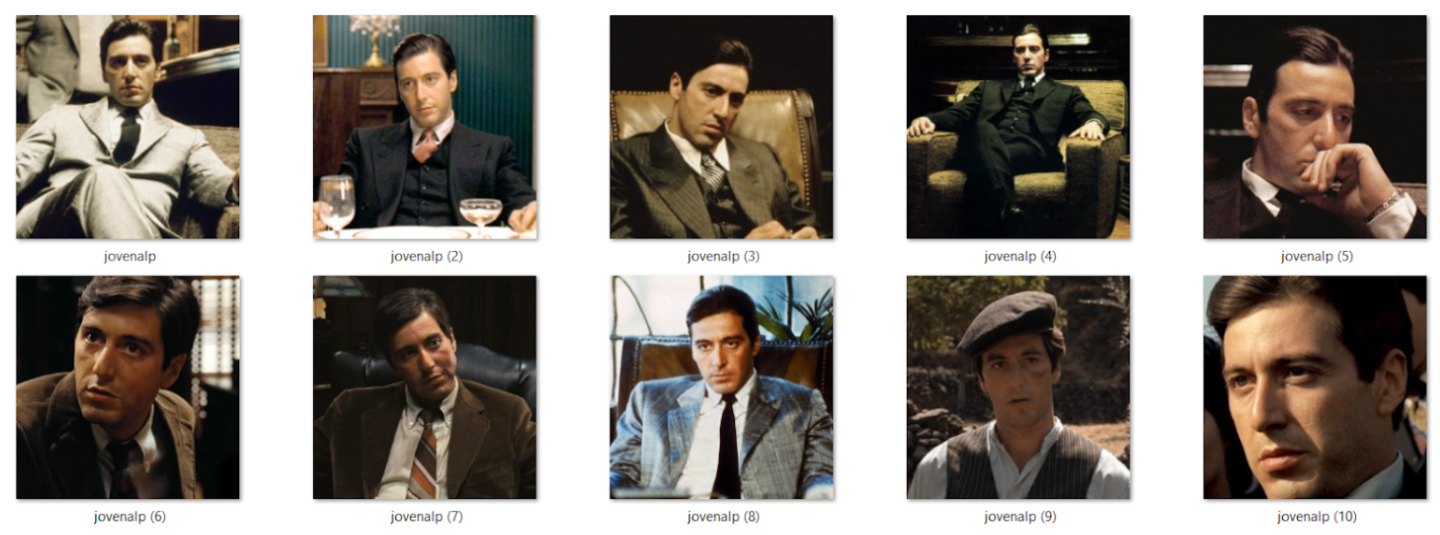
\includegraphics[width = 1
	\textwidth]{Imagenes/Vectorial/dataset_jovenalp.png}
	\caption{Dataset seleccionado para el entrenamiento con Juan de joven}
	\label{fig:datasetjovenalp}
\end{figure}

Tal y como lo hemos dispuesto, el capítulo 1 del libro de vida está compuesto por una serie de recuerdos que representan los acontecimientos más célebres para Juan en sus primeros años. En la tabla \ref*{tab:capitulo1librovida}, especificamos los prompts seleccionados a modo de descripción de sus recuerdos con sus respectivas imágenes como resultado. \\
 
 \begin{table}
 	\centering
 	\begin{tabular}{>{\centering\arraybackslash}m{5cm} >{\arraybackslash}m{5cm}>{\arraybackslash}m{5cm}}
 		\textbf{Recuerdo} & \textbf{Prompt} & \textbf{Resultado final} \\
 		\hline
 		Recuerdo de Juan de niño y su madre por primera vez en su laboratorio personal & Jovenalp as a child with his mother in a chemical laboratory with a white coat, full detail, high quality, hd & 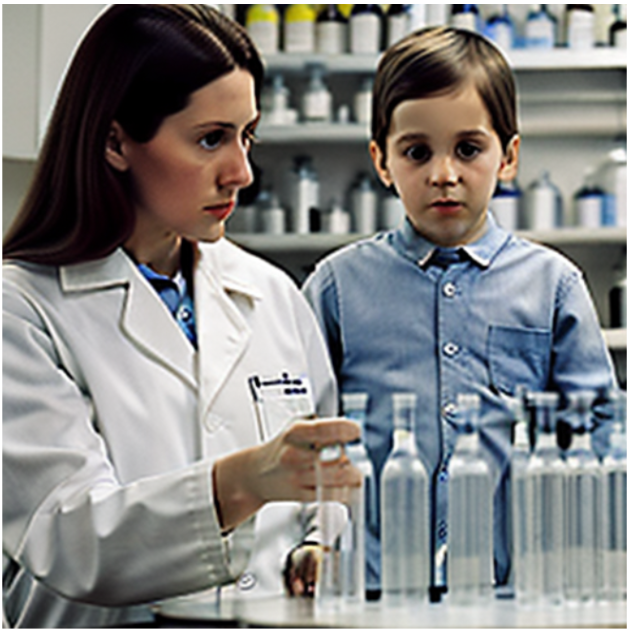
\includegraphics[width = 0.3
 		\textwidth]{Imagenes/Vectorial/alpysumadrelab.png}\\
 		\hline
 		Autorretrato que se hizo Juan de sí mismo &A dumb and sad jovenalp, with sad face. posing 7/11, wearing a leather trench. greyscale style, realistic, pencil sketch & 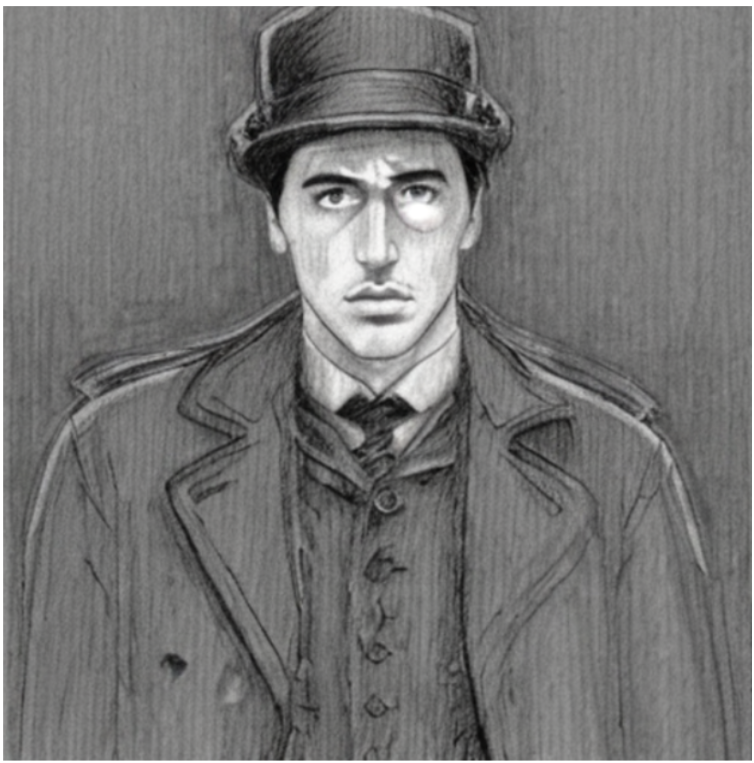
\includegraphics[width = 0.3
 		\textwidth]{Imagenes/Vectorial/autoretratoalp.png}\\
 		\hline
 		La basílica del pueblo donde creció Juan de niño, Colmenar Viejo en navidad & a picture of cvbasil with snow and christmas decoration, high quality, hd & 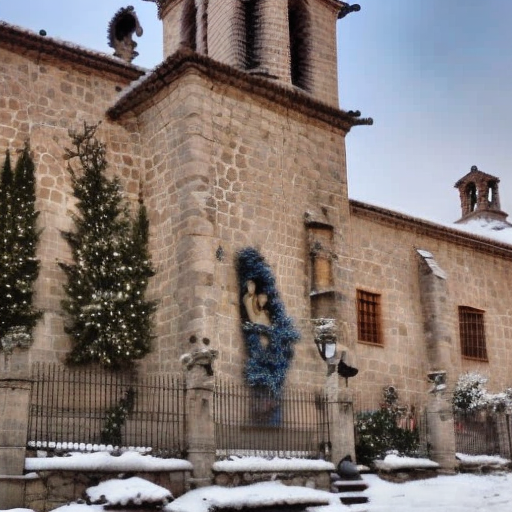
\includegraphics[width = 0.3
 		\textwidth]{Imagenes/Vectorial/colmewinter.png}\\
 		\hline
 		Juan en el jardin de su casa vestido de traje para su primera entrevista de trabajo & jovenalp gentleman in light brown pinstripe double breasted suit, standing in a park & 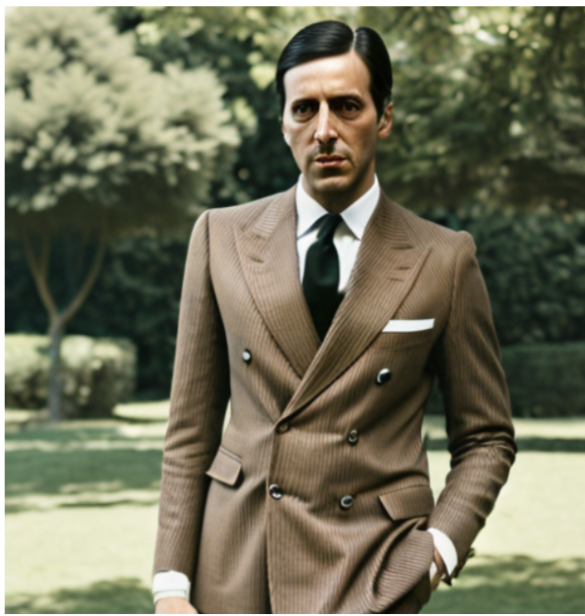
\includegraphics[width = 0.3
 		\textwidth]{Imagenes/Vectorial/jovenalptraje.png}\\
 		\hline
 	\end{tabular}
 	\caption{Tabla de resultados obtenidos del Capítulo 1 de juventud del paciente}
 	\label{tab:capitulo1librovida}
 \end{table}


\section{Fase de la vida 2: Adultez}
Continuando con la vida de Juan en su etapa adulta, consiguió un trabajo como químico en un laboratorio de investigación en la capital. Por ello, decidió mudarse a la capital ya que siempre le gustó la vida en la ciudad. Finalmente, terminó comprándose un piso en el Paseo de la Castellana, concretamente, a 7 minutos andando de las Torres Kio, un elemento de la arquitectura madrileña que le gustaba especialmente. A pesar de que sus años en el equipo de atletismo llegaron a su fin, Juan sigue disfrutando del deporte, aunque de una manera menos intensa y aprovecha sus tiempos libres y de ocio para hacer senderismo por la montaña y poder estar en contacto con la naturaleza. Además, su afición a la pintura nunca la perdió e incluso, fue mejorando su técnica.  

En esta etapa, y para que el libro de vida cobrará más sentido, decimos añadir elementos nuevos para representar los cambios que ocurren en la vida de una persona al cabo de los años. En concreto, hemos entrenado el modelo con las torres Kio de Madrid.

En específico, el token que se le otorgó a esta etapa se llama "adultalp" y el dataset seleccionado son 10 fotos comprendidas entre los 40 y 55 años del actor. En la figura \ref{fig:gan} se pueden apreciar la variedad de las mismas. 

\begin{figure}[!htb]
	\centering
	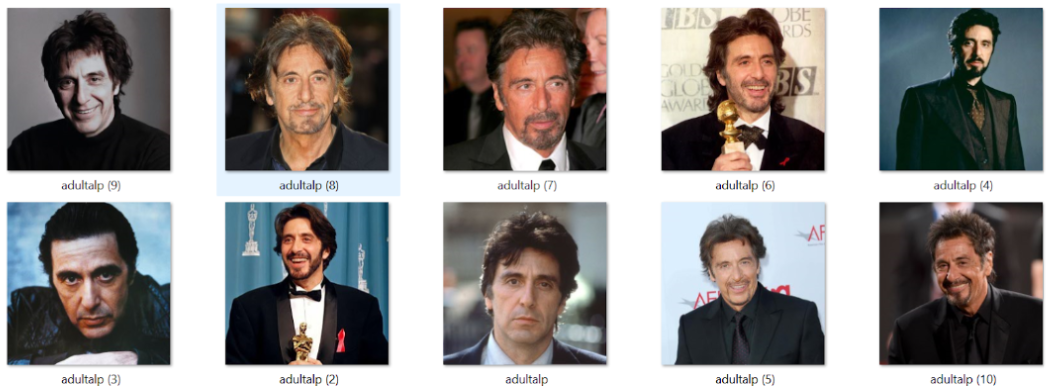
\includegraphics[width = 1
	\textwidth]{Imagenes/Vectorial/dataset_adultalp.png}
	\caption{Dataset seleccionado para el entrenamiento con Juan de adulto}
	\label{fig:datasetadultalp}
\end{figure}

Por otro lado, en la tabla \ref*{tab:capitulo1librovida} están recogidos los resultados de los recuerdos que representamos bajo este nombre y en esta etapa en concreto. \\

 \begin{table}
	\centering
	\begin{tabular}{>{\centering\arraybackslash}m{5cm} >{\arraybackslash}m{5cm}>{\arraybackslash}m{5cm}}
		\textbf{Recuerdo} & \textbf{Prompt} & \textbf{Resultado final} \\
		\hline
		Recuerdo de Juan de niño y su madre por primera vez en su laboratorio personal & Jovenalp as a child with his mother in a chemical laboratory with a white coat, full detail, high quality, hd & 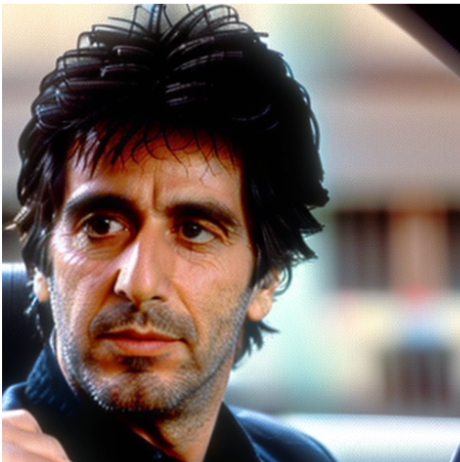
\includegraphics[width = 0.3
		\textwidth]{Imagenes/Vectorial/padultalp.png}\\
		\hline
		Autoretrato que se hizo Juan de sí mismo en su edad adulta &  & 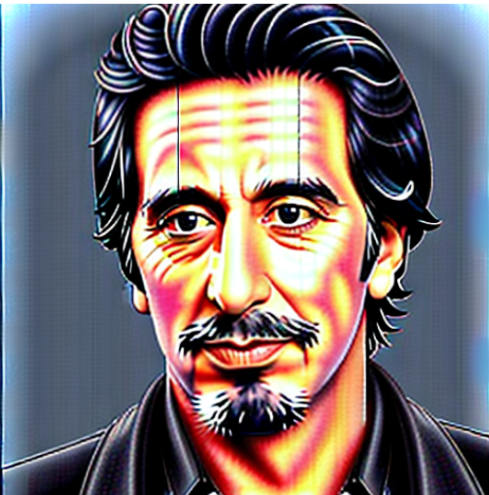
\includegraphics[width = 0.3
		\textwidth]{Imagenes/Vectorial/autorretrato2.png}\\
		\hline
		Juan muy contento haciendo senderismo en la montaña &  & \includegraphics[width = 0.3
		\textwidth]{Imagenes/Vectorial/montaña.png}\\
		\hline
		Juan en el laboratorio de su trabajo & serious adultalp in a chemistry laboratory, with a white coat, detailed face, hd & 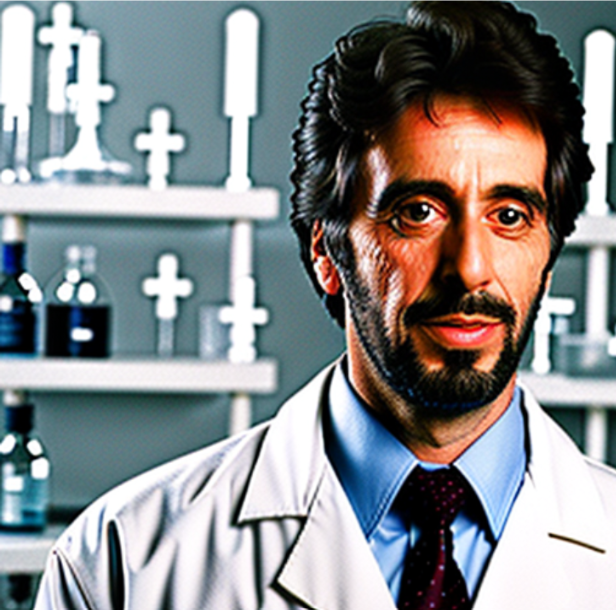
\includegraphics[width = 0.3
		\textwidth]{Imagenes/Vectorial/alplab.png}\\
		\hline
	\end{tabular}
	\caption{Tabla de resultados obtenidos del Capítulo 2 de adultez del paciente}
	\label{tab:capitulo2librovida}
\end{table}
 
\section{Fase de la vida 3: Vejez}
Tras 36 años largos de profesión, Juan decide jubilarse. Debido a su soledad y el deseo que siempre le acompañó de adoptar un fiel compañero, decidió adoptar un perro para hacer sus días más entretenidos y que le pudiese acompañar siempre. Debido a su tiempo libre, Juan se aficionó a la serie televisiva Friends y sus familiares le ayudaron a redecorar su casa con la temática que sigue el salón que aparecía en la serie. Entre otras aficiones, Juan tomó la iniciativa de realizar viajes con el imserso y poder descubrir lugares que no conocía. En sus últimos años, Juan fue optando por actividades algo más sedentarias como leer y jugar al ajedrez hasta que el Alzheimer estuvo tan avanzado que necesitaba estar en un centro atendido por profesionales. En el centro empezó a realizar terapias de reminiscencia junto a su familia y cuidadores y de esta manera, terminó cobrando forma este libro de vida. 

El último conjunto de datos que escogimos comprendía las edades entre los 70 y 84 del actor, más comúnmente conocido como Al Pacino. En la figura \ref{fig:cnn} se puede apreciar más detalladamente las características de las imágenes elegidas. Finalmente, el token asignado fue "80alp". \\

\begin{figure}[!htb]
	\centering
	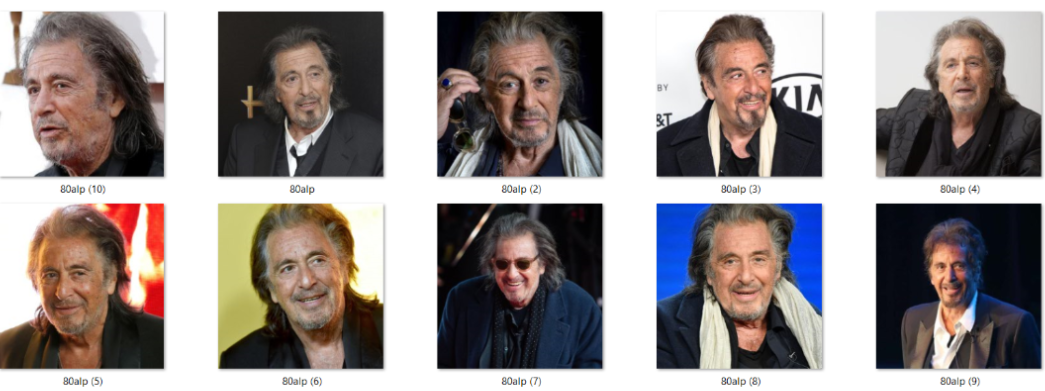
\includegraphics[width = 1
	\textwidth]{Imagenes/Vectorial/dataset_80alp.png}
	\caption{Dataset seleccionado para el entrenamiento con Juan de anciano}
	\label{fig:dataset80alp}
\end{figure}

En la tabla \ref*{tab:capitulo3librovida} podemos apreciar los resultados obtenidos a partir de los últimos recuerdos de Juan, disfrutando de las cosas cotidianas que hace en su día a día a su vez que realizando ejercicios que le fortalecen mentalmente, y por supuesto, en los que se incluyen momentos significativos para él esta etapa. \\


\begin{table}
	\centering
	\begin{tabular}{>{\centering\arraybackslash}m{5cm} >{\arraybackslash}m{5cm}>{\arraybackslash}m{5cm}}
		\textbf{Recuerdo} & \textbf{Prompt} & \textbf{Resultado final} \\
		\hline
		Juan disfrutando de una partida de ajedrez & serious 80alp playing chess, detailed face, long hair, old, hd & 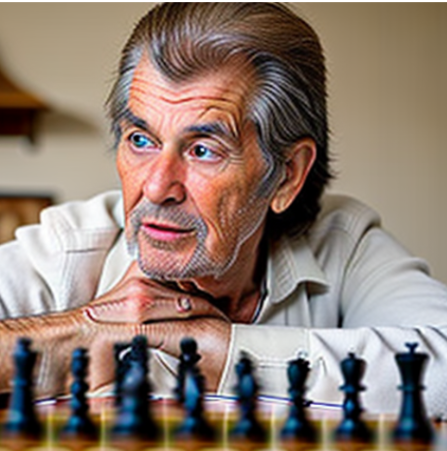
\includegraphics[width = 0.3
		\textwidth]{Imagenes/Vectorial/80alpchess.png}\\
		\hline
		 Juan leyendo su libro favorito en la residencia & serious 80alp reading a book, detailed face, long hair, old, hd & 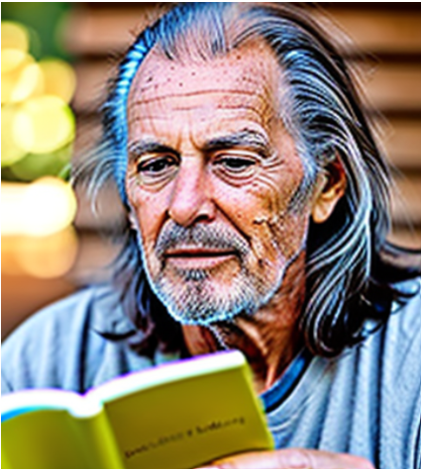
\includegraphics[width = 0.3
		\textwidth]{Imagenes/Vectorial/80alpbook.png}\\
		\hline
		& & 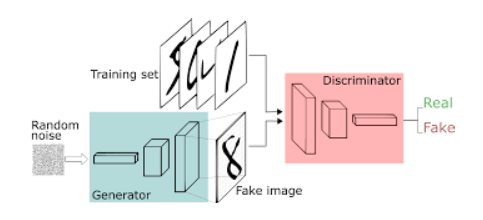
\includegraphics[width = 0.3
		\textwidth]{Imagenes/Vectorial/gan.png}\\
		\hline
		&  & 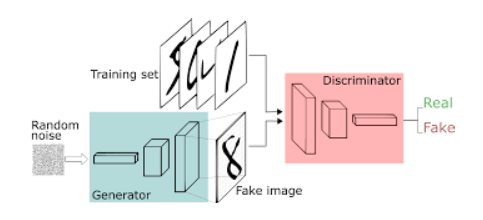
\includegraphics[width = 0.3
		\textwidth]{Imagenes/Vectorial/gan.png}\\
		\hline
	\end{tabular}
	\caption{Tabla de resultados obtenidos del Capítulo 3 de vejez del paciente}
	\label{tab:capitulo3librovida}
\end{table}

Esto muestra cómo responde nuestro modelo a entrenar a una misma persona durante diferentes fases de su vida. Resulta muy útil dados nuestros objetivos iniciales del proyecto, dado que son imágenes que se pueden generar con los elementos que se desee para un libro de vida. Al igual que para el resto de pruebas realizadas, únicamente son necesarias 10 fotografías y se puede apreciar que los resultados son muy buenos y detallados, y lo más importante, se demuestra que el modelo es capaz de generar imágenes completamente diferentes a las que ya existía previamente sobre la persona. Esto es vital, porque de no ser así, el modelo no sería necesario, porque no aportaría ningún valor añadido.